\documentclass{article}

\usepackage{amsthm, amsfonts, amsmath}
\usepackage{graphicx}
\usepackage{fullpage}

\newtheorem{lemma}{Lemma}
\newtheorem{theorem}{Theorem}
\newtheorem{corollary}{Corollary}
\newtheorem{conjecture}{Conjecture}

\begin{document}
	\title{TODO: [Nullity 2 \textit{Lights Out} Boards]}
	\author{William Boyles}
	\date{\today}
	\maketitle
	
	\section{Intro}
	\begin{itemize}
		\item What \textit{Lights Out} is
		\item What quiet patterns are
		\item Certain board sizes require $n^2$ clicks because they have no quiet patterns
		\item Result: For boards where the space of quiet patterns has dimension 2, we can solve this problem exactly.
	\end{itemize}
	
	\section{Solving a 5 x 5}
	The $5 \times 5$ board is the first example with nullity 2.
	\begin{lemma}
		$5 \times 5$ board that is solvable can be done so in no more than 15 clicks.
	\end{lemma}
	\begin{proof}
		Below are the three non-trivial quiet patterns for the $5 \times 5$ board.
		\begin{center}
			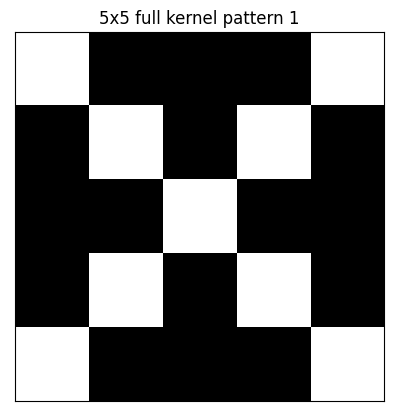
\includegraphics[width=0.49\textwidth]{../../code/serialization/kernels/5x5/full/5x5_kernel_full_1.png}
			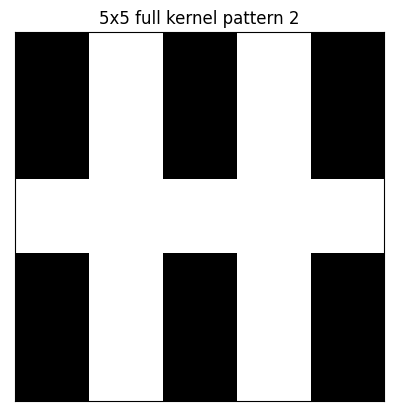
\includegraphics[width=0.49\textwidth]{../../code/serialization/kernels/5x5/full/5x5_kernel_full_2.png}
			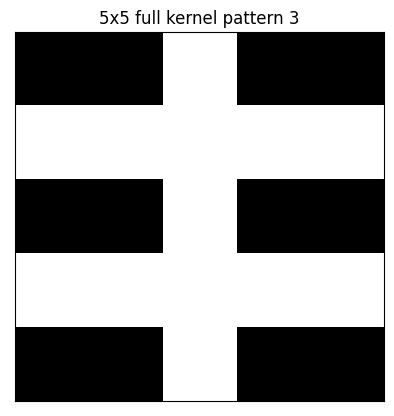
\includegraphics[width=0.49\textwidth]{../../code/serialization/kernels/5x5/full/5x5_kernel_full_3.png}
		\end{center}
		We can divide the squares of the $5 \times 5$ board into four regions based on which quiet patterns they are a part of.
		\begin{center}
			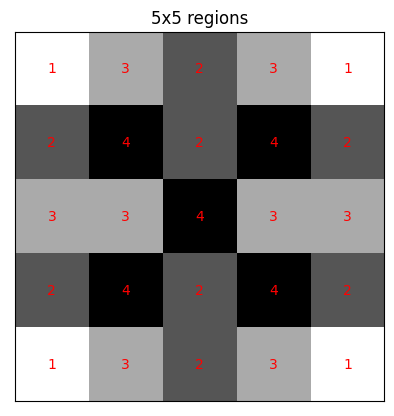
\includegraphics[width=0.49\textwidth]{../../code/serialization/regions/5x5_regions.png}
		\end{center}
		Region 1 is the intersection of quiet patterns 2 and 3; region 2 is the intersection of quiet patterns 1 and 2; region 3 is the intersection of quiet patterns 1 and 3;
		region 4 is in non of the quiet patterns.
		
		Assume that we have a solvable board that requires the maximum number of clicks needed to solve optimally.
		Let $A$ be the number of clicks in the solution in region 1, $B$ in region 2, $C$ in region 3, and $D$ in region 4.
		Then the solution uses $A + B + C + D$ clicks.
		
		If we apply quiet pattern 1, we will get an equivalent solution that uses $A + (8 - B) + (8 - C) + D$ clicks.
		Since we assumed the solution we had to begin with was minimal,
		\begin{equation*}
			A + B + C + D \leq A + (8 - B) + (8 - C) + D.
		\end{equation*}
		Rearranging,
		\begin{equation}
			B + C \leq 8.
		\end{equation}
	
		If we apply quiet pattern 2, we will get an equivalent solution that uses $(4 - A) + (8 - B) + C + D$ clicks.
		Since we assumed the solution we had to begin with was minimal,
		\begin{equation*}
			A + B + C + D \leq (4 - A) + (8 - B) + C + D.
		\end{equation*}
		Rearranging,
		\begin{equation}
			A + B \leq 6.
		\end{equation}
	
		If we apply quiet pattern 3, we will get an equivalent solution that uses $(4 - A) + B + (8 - C) + D$ clicks.
		Since we assumed the solution we had to begin with was minimal,
		\begin{equation*}
			A + B + C + D \leq (4 - A) + B + (8 - C) + D.
		\end{equation*}
		Rearranging,
		\begin{equation}
			A + C \leq 6.
		\end{equation}
	
		In all these constraints we have derived, $D$ is not contrained beyond region 4 containing five buttons.
		Thus, in any board that requires the maximum number of clicks to optimally solve, $D = 5$.
	
		Putting all of these constraints together in matrix form for $A$, $B$, and $C$,
		\begin{equation}
			\begin{bmatrix}
				0 & 1 & 1 \\
				1 & 1 & 0 \\
				1 & 0 & 1
			\end{bmatrix}
			\begin{bmatrix}
				A \\
				B \\
				C
			\end{bmatrix}
			\leq
			\begin{bmatrix}
				8 \\
				6 \\
				6
			\end{bmatrix}.
		\end{equation}
		Clearly, if these constraints were tight with $A$, $B$, and $C$ as integers, than we have a maximal optimal solution.
		Row reducing, we can see that
		\begin{equation*}
			\begin{bmatrix}
				A \\
				B \\
				C
			\end{bmatrix}
			=
			\begin{bmatrix}
				2 \\
				4 \\
				4
			\end{bmatrix}
		\end{equation*}
		is the solution to the tight constraints and has all variables as integers like required.
		Thus, it describes a maximal optimal solution.
		So, a maximal optimal solution uses no more than $A + B + C + D = 2 + 4 + 4 + 5 = 15$ clicks.
	\end{proof}

	\section{Extending to Larger Boards}
	The $5 \times 5$ kernel patterns have a nice property that because that the same buttons are pushed on the top/bottom and left/right edges, they tile to make kernel patterns on larger boards, specifically those of size $6k + 5 \times 6k + 5$, where $k$ is an integer at least 0.
	For example, notice how the kernel patterns on the $17 \times 17$ board ($k = 2$) are the same patterns from the $5 \times 5$ board repeated 3 times in the vertical and horizontal directions.
	\begin{center}
		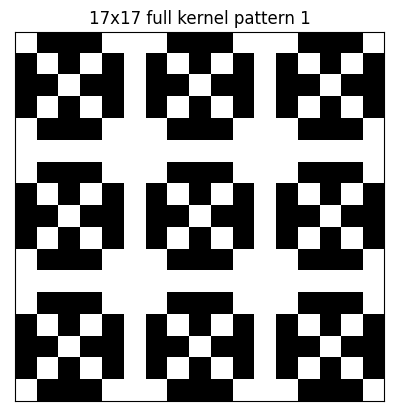
\includegraphics[width=0.49\textwidth]{../../code/serialization/kernels/17x17/full/17x17_kernel_full_1.png}
		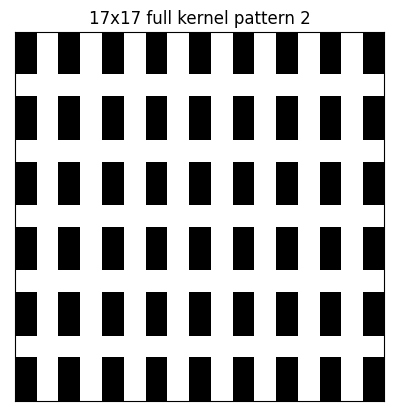
\includegraphics[width=0.49\textwidth]{../../code/serialization/kernels/17x17/full/17x17_kernel_full_2.png}
		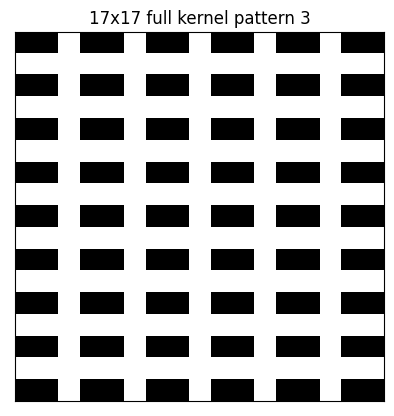
\includegraphics[width=0.49\textwidth]{../../code/serialization/kernels/17x17/full/17x17_kernel_full_3.png}
	\end{center}
	Thus, we can apply the same proof technique from the $5 \time 5$ board to get an upper bound of all boards of size $6k + 5 \times 6k + 5$.
	
	\begin{theorem}
		Let $k$ be an integer at least 0.
		Then a solvable $6k + 5 \times 6k + 5$ board can be solved in no more than $21k^2 + 40k + 15$ clicks.
	\end{theorem}
	\begin{proof}
		As shown above, the three non-trivial quiet patterns of a $5 \times 5$ board will tile a $6k + 5 \times 6k + 5$ board.
		Thus, we can divide the larger board into the same four regions where region 1 has $4(k+1)^2$ lights, regions 2 and 3 both have $8(k+1)^2$ lights, and region 4 has the remaining $5(k+1)^2 + 11k^2 + 10k$ lights.
		Applying the three non-trivial quiet patterns and rearranging into matrix form, we get that $D$ is unconstrained to $5(k+1)^2 + 11k^2 + 10k$, and
		\begin{equation}
			\begin{bmatrix}
				0 & 1 & 1 \\
				1 & 1 & 0 \\
				1 & 0 & 1 
			\end{bmatrix}
			\begin{bmatrix}
				A \\
				B \\
				C
			\end{bmatrix}
			\leq
			\begin{bmatrix}
				8 \\
				6 \\
				6
			\end{bmatrix}(k+1)^2.
		\end{equation}
		So,
		\begin{equation*}
			\begin{bmatrix}
				A \\
				B \\
				C
			\end{bmatrix}
			=
			\begin{bmatrix}
				2 \\
				4 \\
				4
			\end{bmatrix}(k+1)^2.
		\end{equation*}
		Therefore, $A + B + C + D = 2(k+1)^2 + 4(k+1)^2 +  4(k+1)^2 + 5(k+1)^2 + 11k^2 + 10k = 15(k+1)^2 + 11k^2 + 10k = 26k^2 + 40k + 15$.
	\end{proof}

	We can now establish some corollaries
	\begin{corollary}
		All boards of size $6k + 5 \times 6k + 5$ have nullity at least 2.
	\end{corollary}
	\begin{proof}
		We've already shown that the three tiling quiet patterns much exist on all boards of size $6k + 5 \times 6k + 5$.
		The third quiet pattern is the sum for the other two, so these quiet patterns form a space of dimension 2.
	\end{proof}

	\begin{corollary}
		This bound is tight for boards with nullity 2.
	\end{corollary}
	\begin{proof}
		If the board in question only has a null space of dimension 2, then the upper bound proof fully describes all possible equivalent solutions.
	\end{proof}

	The $5 \times 5$, $17 \times 17$, $41 \times 41$, $53 \times 53$, $77 \times 77$, and $113 \times 113$ boards are the boards of size $6k+5$ with nullity 2.
	Thus applying the corollary, they can be solved in no more than 15, 199, 1191, 1999, 4239, and 9159 clicks.
	
	\begin{corollary}
		Let $d(n)$ be the nullity of an $n \times n$ board.
		Then for all integers $a \geq 2$ and $k \geq 0$,
		\begin{equation*}
			d(ak + a - 1) \geq d(a-1).
		\end{equation*}
	\end{corollary}
	\begin{proof}
		Choose any quiet pattern on an $a-1 \times a-1$ board.
		Reflect the pattern $k$ times horizontally and vertically, adding width one spaces between each reflected board.
		This will form a quiet pattern of size $ak + a-1 \times ak + a-1$.
		We can do this reflection operation with all $d(a-1)$ independent quiet patterns to form $d(a-1)$ independent quiet patterns on the larger boards.
	\end{proof}
	
	\section{Conjectures}
	\begin{conjecture}
		If an $n \times n$ board has nullity 2, then $n \equiv 5 \mod 6$.
	\end{conjecture}

	Although we only examined the 5 modulo 6 case here, we can convert all board sizes into an integer programming problem.
	This does not bode well for being able to find solutions to arbitrary boards.
	\begin{conjecture}
		The proof technique of assuming our integer program can be solved with all constraints tight will only work for boards with nullity 2, none higher.
	\end{conjecture}

	This isn't really a formal conjecture that can be proven correct or incorrect, but
	\begin{conjecture}
		If we do manage to solve other nullity boards in a generalized (non brute-force) way like our approach for the 5x5, we'll be able to use a similar tiling argument to establish upper bounds.
	\end{conjecture}
\end{document}